\documentclass[a4paper]{article}
\usepackage[a4paper,top=3cm,bottom=2cm,left=3cm,right=3cm,marginparwidth=1.75cm]{geometry}

% A few common packages

\usepackage{amsthm}
\usepackage{array}
\usepackage{graphicx}
\usepackage[numbers]{natbib}
\usepackage{relsize}
\usepackage[titletoc]{appendix}

% Some other useful packages
\usepackage{caption}
\usepackage{subcaption}  % \begin{subfigure}...\end{subfigure} within figure
\usepackage{multirow}
\usepackage{tabularx}
\usepackage[section]{placeins}
\newcolumntype{M}[1]{>{\centering\arraybackslash}m{#1}}
\usepackage[utf8]{inputenc}
\title{The Simulated 1-D Reflected Shock Problem using the BGK and ES-BGK Approximations to the Boltzmann Equation}
\author{William Jo}
\date{December 5, 2022}
\usepackage{amsmath}
\usepackage{graphicx}
\usepackage{hyperref}
\newcommand*\GitHubLoc{https://bitbucket.org/williejooooo/semester-project/src/master}
\hypersetup{
    colorlinks=true,
    linkcolor=blue,
    filecolor=magenta,      
    urlcolor=cyan,
    pdftitle={Overleaf Example},
    pdfpagemode=FullScreen,
    }
\begin{document}

\maketitle

\section{Introduction}
This report details the theory and application of a problem using the Bhatnagar-Gross-Krook (BGK) and Ellipsoidal-Statistic BGK (ES-BGK) approximations to the Boltzmann equation for non-equilibrium gas flow. For the semester project, a program used to solve the one-dimensional (1-D) numerical reflected shock problem, which had already been written using the BGK approximation for pseudo-Maxwell (PM) molecules, was modified to include the BGK approximation assuming hard-sphere (HS) molecules and the ES-BGK approximation assuming PM molecules. 

This report shall first discuss the problem setup followed by the methodology behind both BGK and ES-BGK approximations for both HS and PM molecules. A general algorithm to the code is described for both BGK and EGK approximations and results for the 1-D shock problem are discussed following the guidelines given in the semester project handout. The shockwave speed is estimated for both BGK and ES-BGK approximations using PM molecules and compared with the analytical solution for verification and uncertainty.

\section{Problem Setup}
\subsection{1-D Reflected Shock Problem}

\begin{figure}[hbt!]
    \centering
    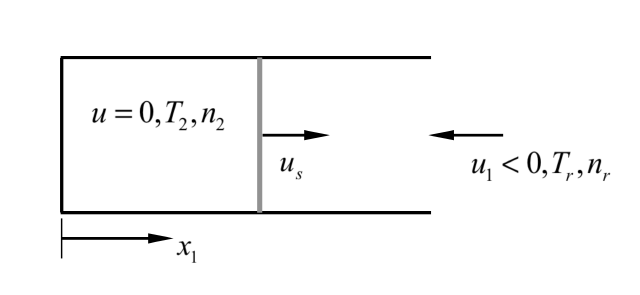
\includegraphics[width=14cm]{imgs/Setup.png}
    \caption{Description of the 1-D Reflected Shock Problem.}
    \label{fig1}
\end{figure}

The objective of this project is to computationally solve the transient flow properties of a reflected shock within a 1-D shock tube, as described in figure \ref{fig1}. The monoatomic gas initially has a uniform scaled velocity of $\hat{u_1} = -1$ and at a scaled time of $\hat{t} = 0$, a reflected wall is inserted at $\hat{x_1} = 0$. The inflow conditions for scaled number density $\hat{n} = 1$ and the scaled temperature $\hat{T} = 1$. The Knudsen number for this flow is $Kn = 1$ corresponding to the reference velocity $\eta_{ref} = (kT_{ref}/m)^{1/2}$ and the reference mean free path to be $\lambda = 1/(n_{ref}\sigma_{ref})$.

\subsection{Discretization of the 1-D Domain}
The total length of the computational domain is $\hat{x}_1 = 250$ and the scaled $x$-distance between discrete points is of size $\alpha_x$. In this 1-D shock problem, the quantity $\alpha_x = 0.5$, giving a total of $500$ space points along the $x$-axis discretizing the 1-D domain. To solve the Boltzmann equation, there must exist a three dimensional (3D) velocity space within each space point in the 1-D physical space domain. The velocity space domain ranges from $\hat{\eta}_1 = [-7,7]$, $\hat{\eta}_2 = [-7,7]$, $\hat{\eta}_3 = [-7,7]$, where $\hat{\eta}_1$ is the velocity space in the $x$-direction, $\hat{\eta}_2$ is the velocity space in the $y$-direction, and $\hat{\eta}_3$ is the velocity space in the $z$-direction. The velocity space within each physical space point is broken up to 21 velocity space points in each direction, with scaled $\eta$ distance between discrete points is of size $\beta_v$. In this 1-D shock problem, the quantity $\beta_v = 0.7$, giving a total of $23^3 = 9,261$ velocity space points to describe one single physical space point. In total to describe the 1-D domain, there must be $500 \times 23^3 = 6,083,500$ data values stored per time step. A simplified figure detailing the discretization of the 1-D physical space domain $\hat{x}$ and the velocity space domain for each physical space point is described in figure \ref{fig2}.

\begin{figure}[hbt!]
    \centering
    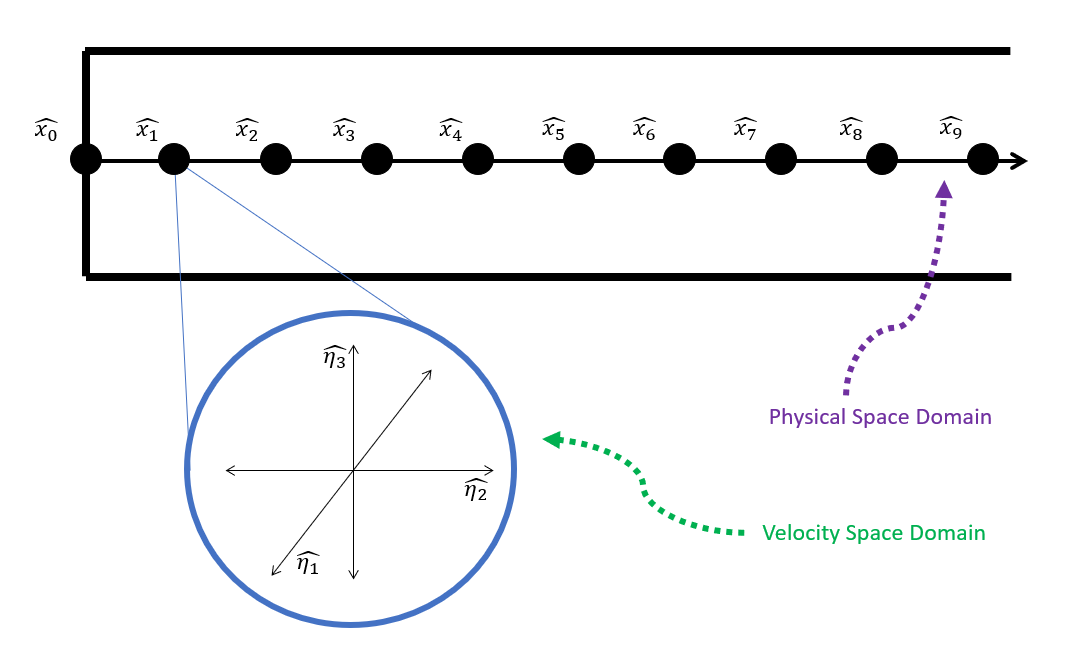
\includegraphics[width=14cm]{imgs/Domain_Description.png}
    \caption{\centering Discretization of the 1-D physical space domain $\hat{x}$, where each physical space point contains a velocity space domain $\hat{\eta}$.}
    \label{fig2}
\end{figure}

\section{Methodology}
The main goal of this project is to modify the existing 1-D reflected shock computation to not only include the BGK approximation, but also to include the BGK approximation using a hard-shell approximation for molecules and the ES-BGK approximation for pseudo-Maxwell molecules.  The following section will discuss the methodology and modifications used to update this flow solver.

\subsection{Governing Equation}
The Boltzmann equation for gas flow not in thermal equilibrium can be written as the following equation below in Einstein notation \cite{vincenti1975introduction}.
\begin{equation}
    \dfrac{\partial}{\partial t}(nf) + \eta_j \dfrac{\partial}{\partial x_j} (nf)  + \dfrac{\partial}{\partial \eta_j} (F_j nf) = \left[\dfrac{\partial}{\partial t}  (nf) \right]_{coll}
\end{equation}
The collision term on the right hand side of the above equation can be written as the following integral per Vincenti et al. (1966) \cite{vincenti1975introduction}. The term in the equation $f(\eta_i)f(\xi_i)$ represents the collision between molecules with velocities $\eta_i$ and $\xi_i$ and the term $f(\eta_i')f(\xi_i')$ representing inverse collisions between molecules of velocities $\eta_i'$ and $\xi_i'$. 
\begin{equation}
    \left[\dfrac{\partial}{\partial t} (nf)\right]_{coll} = \int^{\,\,\,\infty}_{-\infty} \int_{dP_{\eta}} n^2 [f(\eta_i')f(\xi_i') - f(\eta_i)f(\xi_i)]g\,dP_{\eta}\,dV_\xi
\end{equation}
For equilibrium, each depleting collision must be exactly balanced by its inverse. This means that the term in the integrand $f(\eta_i')f(\xi_i') - f(\eta_i)f(\xi_i) = 0$. At equilibrium, the Boltzmann equation becomes:
\begin{equation}
    \dfrac{\partial}{\partial t}(nf) + \eta_j \dfrac{\partial}{\partial x_j} (nf)  + \dfrac{\partial}{\partial \eta_j} (F_j nf) = 0
\end{equation}
However for a shock, the system would not be in equilibrium so the term on the right hand side of the Boltzmann equation must be non-zero. 

\subsection{BGK Collision Model}
To simplify the right hand side of the Boltzmann equation, a solution has been described by Bhatnagar, Gross, and Krook (1954) that eliminates the complexities of the nonlinear integral form \cite{bhatnagar1954model}. The collision integral is replaced by the following equation:
\begin{equation}
    \left[\dfrac{\partial}{\partial t} (nf)\right]_{coll} = n \nu (f_M - f)
\end{equation}
The full term implemented in the Boltzmann equation is shown below:
\begin{equation}
    \dfrac{\partial}{\partial t}(nf) + \eta_j \dfrac{\partial}{\partial x_j} (nf)  + \dfrac{\partial}{\partial \eta_j} (F_j nf) = n \nu (f_M - f)
\end{equation}
The term $f_M$ represents the Maxwellian distribution expressed in terms of the local mean velocity and the local temperature. The term $\nu$ is the collision frequency and directly proportional to number density $n$. If the BGK equation were non-dimensionalized with the term $\hat{n} = n/n_{ref}$, $\hat{t} = t\eta_i/L$, etc., and assuming that $\hat{\varphi} = \hat{n}\hat{f}$ without any body forces $F_j$, the following non-dimensionalization of the Boltzmann equation is achieved:
\begin{equation}
    \dfrac{\partial}{\partial \hat{t}}(\hat{\varphi}) + \eta_j \dfrac{\partial}{\partial \hat{x}_j} (\hat{\varphi})  = \dfrac{1}{Kn}\hat{\nu} (\hat{\varphi}_M - \hat{\varphi})
\end{equation}
\subsection{ES-BGK Collision Model}
The governing equations for the ES-BGK equation is similar to the BGK equation. However, the quantity for the Maxwellian $\hat{\varphi}_M$ is replaced by a term $\hat{\psi} '$ that has to be solved. This section will discuss the algorithm to solving the ES-BGK equations following the steps from Holway (1966) and Gallis and Torczynski (2011) \cite{holway1966new}, \cite{gallis2011investigation}. The first step is to find the solution of $\hat{M}_{ij}$, described below:
\begin{equation}
    \hat{M}_{ij} = \dfrac{1}{\hat{n}} {\int_{V_{\eta}}} \hat{c}_{i} \hat{c}_{j} \hat{\varphi}dV_{\eta}
\end{equation}
Using the value of $\hat{M}_{ij}$, the value of $\hat{\Lambda}_{ij}$ can be determined from the following equation:
\begin{equation}
   \hat{\Lambda}_{ij} = \hat{T}\delta_{ij} + \Tilde{\lambda}\hat{M}_{ij} 
\end{equation}
Noting that the value of $\Tilde{\lambda} = -1/2$, the matrix $\hat{\Lambda}_{ij}$ is a diagonal matrix consisting only the variables along the diagonal: $\hat{\Lambda}_{11}$, $\hat{\Lambda}_{22}$, $\hat{\Lambda}_{33}$. The determinant of $\hat{\Lambda}_{ij}$ becomes $|\hat{\Lambda}| = \hat{\Lambda}_{11}\hat{\Lambda}_{22}\hat{\Lambda}_{33}$. The inverse of the matrix $\hat{\varepsilon}_{ij}$ becomes just $\hat{\varepsilon}_{ij} = 1/\hat{\Lambda}_{ij}$ for only values along the diagonal ($i=j$). Using these variables above, the value of $\psi '$ can be determined:
\begin{equation}
    \hat{\psi} ' = \dfrac{\hat{n}}{(2\pi)^{3/2}} \dfrac{1}{|\hat{\Lambda}|^{1/2}} exp\left(-\dfrac{1}{2}\hat{c}_i \hat{\varepsilon}_{ij} \hat{c}_j \right)
\end{equation}
The Boltzmann equation will then become the following with the ES-BGK collision model implemented:
\begin{equation}
    \dfrac{\partial}{\partial \hat{t}}(\hat{\varphi}) + \hat{\eta}_j \dfrac{\partial}{\partial \hat{x}_j} (\hat{\varphi})  = \dfrac{1}{Kn}\hat{\nu} (\hat{\psi} ' - \hat{\varphi})
\end{equation}

\subsection{Hard Shell Models for BGK and ES-BGK Collision Models}
For pseudo-Maxwell molecules, the value of $\hat{\nu}$ is represented by the following equation \cite{Varghese_BGK}:
\begin{equation}
    \hat{\nu}_{pM} = \hat{n}
\end{equation}
For hard-spheres, the value of $\hat{\nu}$ is represented by the following equation \cite{Varghese_BGK}:
\begin{equation}
    \hat{\nu}_{ES} = \hat{n}\hat{T}^{1/2}
\end{equation}
The normalization of the right hand side of the Boltzmann equation introduces a term $\hat{K}$ which represents the scaling. To compare the BGK and ES-BGK models, the term $\hat{K}$ cannot be ignored. The BGK equation with $\hat{K}$ becomes:
\begin{equation}
    \dfrac{\partial}{\partial \hat{t}}(\hat{\varphi}) + \hat{\eta}_j \dfrac{\partial}{\partial \hat{x}_j} (\hat{\varphi})  = \dfrac{\hat{K}_{BGK}}{Kn}\hat{\nu} (\hat{\varphi}_M - \hat{\varphi})
\end{equation}
The ES-BGK equation with $\hat{K}$ also becomes:
\begin{equation}
    \dfrac{\partial}{\partial \hat{t}}(\hat{\varphi}) + \hat{\eta}_j \dfrac{\partial}{\partial \hat{x}_j} (\hat{\varphi})  = \dfrac{\hat{K}_{ES}}{Kn}\hat{\nu} (\hat{\psi} ' - \hat{\varphi})
\end{equation}
The solution of $\hat{K}$ for both BGK and ES-BGK collision models depends on whether or not the molecules are represented as hard spheres or pseudo-Maxwell molecules. From literature, the following equations represent the value of $\hat{K}$ for the BGK model \cite{Varghese_BGK}:
\begin{equation}
    \hat{K}_{BGK, pM} = \dfrac{2}{\sqrt{\pi}} \,\,\,\,\,\,\, \hat{K}_{BGK, HS} = \dfrac{8}{5} \sqrt{\dfrac{2}{\pi}} \hat{T}^{1/2}
\end{equation}
From literature, the following equations represent the value of $\hat{K}$ for the ES-BGK model:
\begin{equation}
    \hat{K}_{ES, pM} = \dfrac{4}{3\sqrt{\pi}} \,\,\,\,\,\,\, \hat{K}_{ES, HS} = \dfrac{16}{15} \sqrt{\dfrac{2}{\pi}} \hat{T}^{1/2}
\end{equation}

\subsection{Numerical Model}
The BGK approximation the the Boltzmann Equation is given as the following equation:
\begin{equation}
    \dfrac{\partial}{\partial \hat{t}}(\hat{\varphi}) + \hat{\eta}_j \dfrac{\partial}{\partial \hat{x}_j} (\hat{\varphi})  = \dfrac{\hat{K}}{Kn}\hat{\nu} (\hat{\varphi}_M - \hat{\varphi})
\end{equation}
The spatial derivative is moved to the right hand side, attaining the following relation:
\begin{equation}
    \dfrac{\partial}{\partial \hat{t}}(\hat{\varphi})   = \dfrac{\hat{K}}{Kn}\hat{\nu} (\hat{\varphi}_M - \hat{\varphi}) - \hat{\eta}_j \dfrac{\partial}{\partial \hat{x}_j} (\hat{\varphi})
\end{equation}
The partial differential equation above is in the form of the following equation, where $f_0$ and $f_1$ are operators of $\hat{\varphi}$:
\begin{equation}
    \dfrac{\partial\hat{\varphi}}{\partial \hat{t}} = f_0(\hat{\varphi}) + f_1(\hat{\varphi})
\end{equation}
The time derivative can be discretized to the following form:
\begin{equation}
   \dfrac{\partial \hat{\varphi}}{\partial \hat{t}} = \dfrac{\hat{\varphi}^{n+1} - \hat{\varphi}^{n}}{\Delta \hat{t}} 
\end{equation}
A split can be formed from $f_0$ and $f_1$ using the time discretization above, following that of Langtangen and Linge (2017) \cite{langtangen2017finite}:
\begin{equation}
    \dfrac{\hat{\varphi}^{*} - \hat{\varphi}^{n}}{\Delta \hat{t}} = f_0(\hat{\varphi}^n)
\end{equation}
\begin{equation}
    \dfrac{\hat{\varphi}^{n+1} - \hat{\varphi}^{*}}{\Delta \hat{t}} = f_1(\hat{\varphi}^*)
\end{equation}
Using the BGK equation, the following first-order splitting form is achieved:
\begin{equation}
    \dfrac{\hat{\varphi}^{*}_j - \hat{\varphi}^{n}_j}{\Delta \hat{t}} =\hat{\nu} \hat{K}(\hat{\varphi}_M - \hat{\varphi}^n_j) 
\end{equation}
\begin{equation}
    \dfrac{\hat{\varphi}^{n+1}_j - \hat{\varphi}^{*}_j}{\Delta \hat{t}} = -\hat{\eta}_j \left(\dfrac{\hat{\varphi}^*_{j} - \hat{\varphi}^*_{j-1}}{\Delta \hat{x}}\right)
\end{equation}
To solve for $\hat{\varphi}^{n+1}_j$ at the next time step,  the computation must initially solve for $\hat{\varphi_j}^*$ at the current time step for all points $j$ in the 1-D physical space domain:
\begin{equation}
    \hat{\varphi}^{*}_j = \hat{\varphi}^{n}_j + \Delta\hat{t} \, \hat{\nu} \hat{K}(\hat{\varphi}_M - \hat{\varphi}^n_j) 
\end{equation}
Using $\hat{\varphi_j}^*$ as the input for the second splitted equation, the computation can then solve for $\hat{\varphi}^{n+1}_j$:
\begin{equation}
    \hat{\varphi}^{n+1}_j = \hat{\varphi}^{*}_j - {\Delta \hat{t}}\hat{\eta}_j \left(\dfrac{\hat{\varphi}^*_{j} - \hat{\varphi}^*_{j-1}}{\Delta \hat{x}}\right)
\end{equation}
The term $\eta_j \Delta \hat{t}/\Delta \hat{x}$ is also known as the Courant–Friedrichs–Lewy (CFL) number, which has to meet the following condition for first-order explicit convergence:
\begin{equation}
    CFL \leq 1 
\end{equation}
The splitting process is used as well to solve for the ES-BGK equations, though it is more computationally involved as $\hat{\varphi}_M$ is replaced by $\hat{\psi}'$, a value to be found that is more computationally involved than the computation of $\hat{\varphi}_M$. Therefore, only the first splitted equation will differ for the ES-BGK approximation and thus become:
\begin{equation}
    \hat{\varphi}^{*}_j = \hat{\varphi}^{n}_j + \Delta\hat{t} \, \hat{\nu} \hat{K} (\hat{\psi}' - \hat{\varphi}^n_j) 
\end{equation}
\subsection{Derivation of Flow Properties from $\hat{\varphi}$}
Using $\hat{\varphi}$, the values for the number density ($\hat{n}$), flow velocity ($\hat{u}_x$), temperature ($\hat{T}$), heat fluxes ($\hat{q}_x$), and viscous stresses ($\hat{\tau}_{xx}$ and $\hat{\tau}_{xy}$) can be derived following that of Vincenti et al. (1966) \cite{vincenti1975introduction}. The definition of the average is used to solve for the number density and velocity of the flow. The definition of the average is as follows:
\begin{equation}
    \Bar{Q} = \int_{V_{\hat{\eta}}} Q\,\hat{f}_{\hat{\eta}}\,dV_{\hat{\eta}}
\end{equation}
The averaged normalized number density can be found with the following integral:
\begin{equation}
    \hat{n}_{avg} = \int_{V_{\hat{\eta}}} \hat{n}\,\hat{f}_{\hat{\eta}}\,dV_{\hat{\eta}}
\end{equation}
Recalling that $\hat{\varphi} = \hat{n} \hat{f}_{\hat{\eta}}$, the averaged normalized number density is found to be:
\begin{equation}
    \hat{n}_{avg} = \int_{V_{\hat{\eta}}} \hat{\varphi}\,dV_{\hat{\eta}}
\end{equation}
The volume integral can be discretized as the following series of sums, where $i,j,k$ are the indices representing the 3-D velocity space, and $ns$ is the index representing the 1-D physical space:
\begin{equation}
    \hat{n}(ns) = \beta_v^3 \sum_k \sum_j \sum_i \hat{\varphi}(i,j,k,ns)
\end{equation}
Similarly, the averaged normalized velocity can be found with the following integral:
\begin{equation}
    \hat{u}_{avg} = \int_{V_{\hat{\eta}}} \hat{\eta}_i\,\hat{f}_{\hat{\eta}}\,dV_{\hat{\eta}}
\end{equation}
Substituting $\hat{\varphi}$ in place of $\hat{f}_{\hat{\eta}}$, the following equation is obtained for the averaged velocity.
\begin{equation}
    \hat{u}_{avg} = \dfrac{1}{\hat{n}}\int_{V_{\hat{\eta}}} \hat{\eta}_i\,\hat{\varphi}\,dV_{\hat{\eta}}
\end{equation}
The volume integral can also be discretized as the following series of sums:
\begin{equation}
    \hat{u}(ns) = \dfrac{\beta_v^3}{\hat{n}(ns)} \sum_k \sum_j \sum_i \hat{\eta}_i\hat{\varphi}(i,j,k,ns) 
\end{equation}
The term $\hat{\eta}_i$ represents the velocity space in the $x$-direction, and by definition $\hat{\eta}_i = \beta_v i$. The discretization to solve for the $\hat{u}$ velocity becomes:
\begin{equation}
    \hat{u}(ns) = \dfrac{\beta_v^3}{\hat{n}(ns)} \sum_k \sum_j \sum_i (\beta_v i)\hat{\varphi}(i,j,k,ns) 
\end{equation}
The integral for normalized temperature is the following equation:
\begin{equation}
    \hat{T} = \dfrac{1}{3} \int_{V_{\hat{\eta}}} \hat{C}^2 \hat{f}_{\hat{\eta}} \,dV_{\hat{\eta}} = \dfrac{1}{3\hat{n}} \int_{V_{\hat{\eta}}} \hat{C} \hat{\varphi} \,dV_{\hat{\eta}}
\end{equation}
The velocity $C^2$ can be rewritten as the following equation:
\begin{equation}
    \hat{C}^2 = \hat{c}_i^2 + \hat{c}_j^2 + \hat{c}_k^2 
\end{equation}
From definition, the term $\hat{c}_i = \hat{\eta}_i - \hat{u}_i = \beta_v i -\hat{u}_i $. When represented as a series of sums, the temperature integral becomes:
\begin{equation}
    \hat{T}(ns) = \dfrac{\beta_v^3}{\hat{n}(ns)} \sum_k \sum_j \sum_i \left[(\beta_v i - \hat{u}(ns))^2 + (\beta_v j)^2 + (\beta_v k)^2 \right]\hat{\varphi}(i,j,k,ns)
\end{equation}
The heat flux in the $x$-direction $\hat{q}_x$ is written as the following integral:
\begin{equation}
    \hat{q}_i = \dfrac{1}{2} \int_{V_{\hat{\eta}}} \hat{c_i}^2\hat{C}^2 \hat{\varphi} \,dV_{\hat{\eta}}
\end{equation}
Following a similar process shown in the derivations above, the summation for the heat flux in the $x$-direction is described below:
\begin{equation}
    \hat{q}_x(ns) = \dfrac{\beta_v^3}{2} \sum_k \sum_j \sum_i (\beta_v i - \hat{u}(ns))^2\left[(\beta_v i - \hat{u}(ns))^2 + (\beta_v j)^2 + (\beta_v k)^2 \right]\hat{\varphi}(i,j,k,ns)
\end{equation}
The heat flux in the $y$ and $z$ directions can be written as the following sums:
\begin{equation}
    \hat{q}_y(ns) = \dfrac{\beta_v^3}{2} \sum_k \sum_j \sum_i (\beta_v j)^2\left[(\beta_v i - \hat{u}(ns))^2 + (\beta_v j)^2 + (\beta_v k)^2 \right]\hat{\varphi}(i,j,k,ns)
\end{equation}
\begin{equation}
    \hat{q}_z(ns) = \dfrac{\beta_v^3}{2} \sum_k \sum_j \sum_i (\beta_v k)^2\left[(\beta_v i - \hat{u}(ns))^2 + (\beta_v j)^2 + (\beta_v k)^2 \right]\hat{\varphi}(i,j,k,ns)
\end{equation}
The viscous stresses for $xx$ is written as the following integral:
\begin{equation}
    \hat{\tau}_{ij} = -\int_{V_{\hat{\eta}}} {\hat{c}_i}^{{\,\,\,o}}\hat{c_j} \hat{\varphi} \,dV_{\hat{\eta}}
\end{equation}
It can be noted that the term ${\hat{c}_i}^{{\,\,\,o}}\hat{c_j}$ can be written as the following:
\begin{equation}
    {\hat{c}_i}^{{\,\,\,o}}\hat{c_j} = \hat{c}_i \hat{c}_j - \dfrac{1}{3}\hat{C}^2\delta_{ij}
\end{equation}
In summation form, the integral for the viscous stresses in $11$ is described below. Note that the Kronecker delta $\delta_{ij} = 0$ for $i\neq j$:
\begin{equation}
    \hat{\tau}_{11}(ns) = \beta_v^3 \sum_k \sum_j \sum_i \left(-\left(\beta_v i - u(ns)\right)^2 + \dfrac{1}{3}\left[(\beta_v i - \hat{u}(ns))^2 + (\beta_v j)^2 + (\beta_v k)^2 \right]^2\right) \hat{\varphi}(i,j,k,ns)
\end{equation}
Following a similar process, the viscous stresses in $12$ is described in the summation form below:
\begin{equation}
    \hat{\tau}_{12}(ns) = \beta_v^3 \sum_k \sum_j \sum_i -(\beta_v i - \hat{u}(ns))(\beta_v j)  \hat{\varphi}(i,j,k,ns)
\end{equation}
\newpage
\section{Results}
\subsection{BGK Pseudo-Maxwell Molecules Approximation}
\subsubsection{Scaled Density, Velocity, Temp. Profiles (Part A)}
\begin{figure}[hbt!]
    \centering
    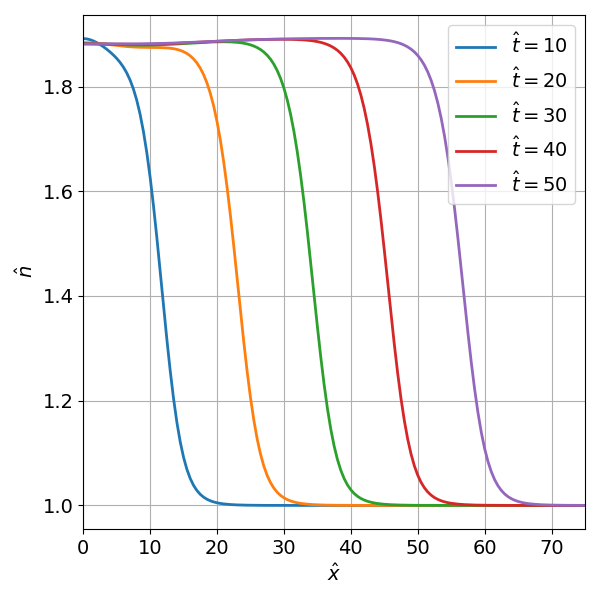
\includegraphics[width=14cm]{plots/problem_a_nd.png}
    \caption{\centering Plot of normalized number density $\hat{n}$ with respect to distance $\hat{x}$ for times $\hat{t} = 10 - 50$ after the main shock has reflected from the wall using inlet speed $\hat{u} = -1$.} 
    \label{problem_a_nd}
\end{figure}
From the plot of normalized number density $\hat{n}$ with respect to distance $\hat{x}$ which is 1-D, it can be seen that the density ratio from number densities obtained ahead and behind the shock rises slightly with each subsequent time step, with the exception of the time step when $\hat{t} = 10$. At $\hat{t} = 10$, the effects of the shock reflecting off the left wall may have still left the domain behind the shock to not have settled completely, and in turn cause a slightly higher number density ratio for the region behind vs. ahead of the shock. It can be seen that after $\hat{t} = 30$, the plot of $
\hat{n}$ vs $\hat{x}$ follow the same plots as $\hat{t} = 40$ and $\hat{t} = 50$, suggesting that the region behind the reflected shock has settled into equilibrium. It is also expected that the shock structure is uniform throughout the time marching, and it can be seen that the downward slopes from an $\hat{n} \approx 1.9$ to $\hat{n} = 1$ are almost identical and spaced evenly apart. 
\clearpage
\begin{figure}[hbt!]
    \centering
    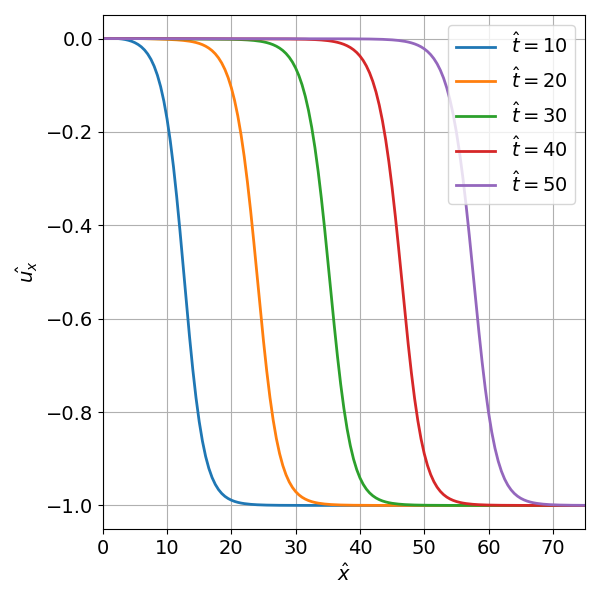
\includegraphics[width=14cm]{plots/problem_a_u.png}
    \caption{\centering Plot of normalized velocity $\hat{u}_x$ with respect to distance $\hat{x}$ for times $\hat{t} = 10 - 50$ after the main shock has reflected from the wall using inlet speed $\hat{u} = -1$.}
    \label{problem_a_U}
\end{figure}

From the plot of normalized number density $\hat{u}$ with respect to distance $\hat{x}$ which is 1-D, it can be seen that the averaged velocity obtained behind the shock is exactly 0. This velocity is expected in the literature after a shock has reflected off a wall. A downwards slope from 0 to a velocity -1 is seen for all times $\hat{t} = 10 - 50$, representing the shock itself. As the distance from the wall increases, it is expected that the velocity of the flow would match that of the inlet speed $\hat{u} = -1$. 

\clearpage
\begin{figure}[hbt!]
    \centering
    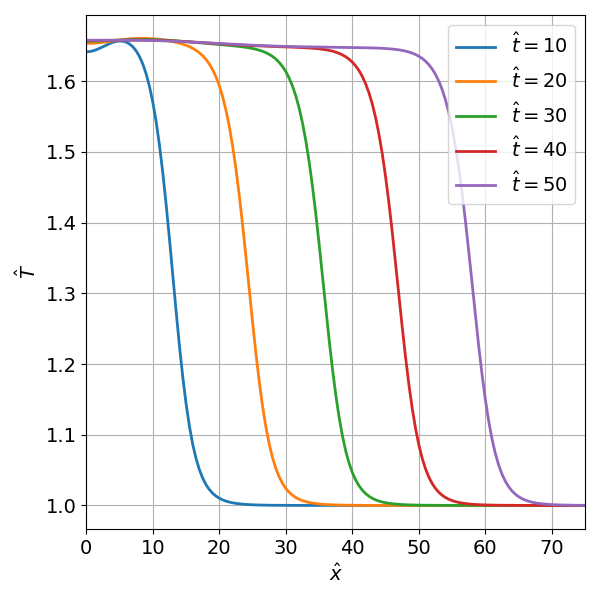
\includegraphics[width=14cm]{plots/problem_a_T.png}
    \caption{\centering Plot of normalized temperature $\hat{T}$ with respect to distance $\hat{x}$ for times $\hat{t} = 10 - 50$ after the main shock has reflected from the wall using inlet speed $\hat{u} = -1$.}
    \label{problem_a_T}
\end{figure}
From the plot of normalized temperature $\hat{T}$ with respect to distance $\hat{x}$ which is 1-D, it can be seen that the temperature ratio from number densities obtained ahead and behind the shock falls slightly with each subsequent time step, with the exception of the time step when $\hat{t} = 10$. Similar to the plot of $\hat{n}$ vs $\hat{x}$, at $\hat{t} = 10$, the effects of the shock reflecting off the left wall may cause the domain trailing the shock to not settle completely, and in turn cause a slightly lower temperature ratio for the region behind vs. ahead of the shock. Again, it can be seen that after $\hat{t} = 30$, the plot of $\hat{T}$ vs $\hat{x}$ follow the same plots as $\hat{t} = 40$ and $\hat{t} = 50$, suggesting that the region behind the reflected shock has settled into equilibrium after this time. It is also expected that the shock structure is uniform throughout the time marching, and it can be seen that the downward slopes from an $\hat{n} \approx 1.7$ to $\hat{n} = 1$ are almost identical and spaced evenly apart. 

\clearpage
\subsubsection{3D Surface Plots of the Distribution Function $\hat{\varphi}$ (Part B)}
\begin{figure}[hbt!]
    \centering
    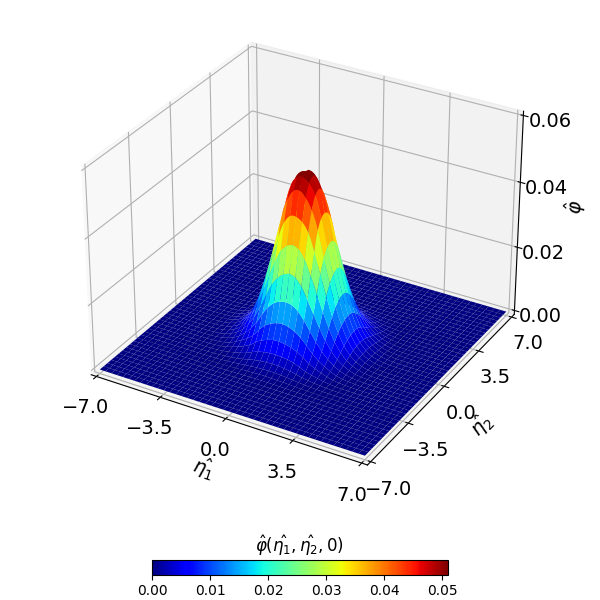
\includegraphics[width=14cm]{plots/problem_b_1.png}
    \caption{\centering 3D plot of the the distribution function $\hat{\varphi}$ at $\hat{\varphi}(\eta_1, \eta_2, 0)$, where $\hat{t} = 40$ and $\hat{x}_1 = 40$.}
    \label{problem_b_1}
\end{figure}
\clearpage
\begin{figure}[hbt!]
    \centering
    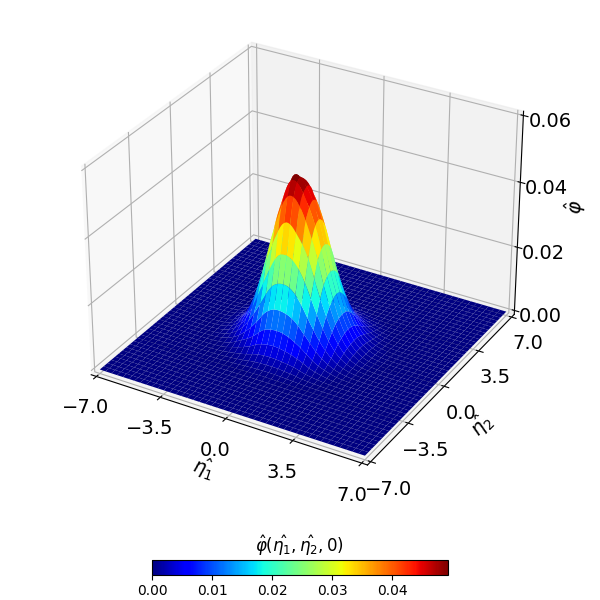
\includegraphics[width=14cm]{plots/problem_b_2.png}
    \caption{\centering 3D plot of the the distribution function $\hat{\varphi}$ at $\hat{\varphi}(\eta_1, \eta_2, 0)$, where $\hat{t} = 40$ and $\hat{x}_1 = 45$.}
    \label{problem_b_2}
\end{figure}
\clearpage
\begin{figure}[hbt!]
    \centering
    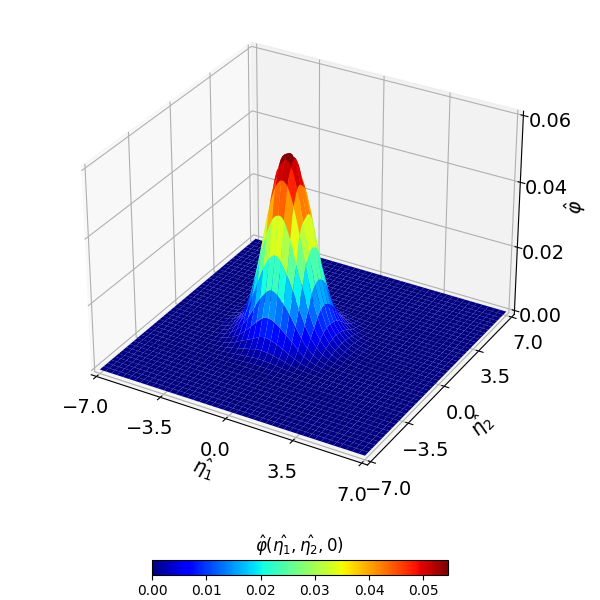
\includegraphics[width=14cm]{plots/problem_b_3.png}
    \caption{\centering  3D plot of the the distribution function $\hat{\varphi}$ at $\hat{\varphi}(\eta_1, \eta_2, 0)$, where $\hat{t} = 40$ and $\hat{x}_1 = 50$.}
    \label{problem_b_3}
\end{figure}
From the three different 3D plots of the distribution function $\hat{\varphi}(\eta_1, \eta_2, 0)$ at $\hat{t} = 40$, it can be seen from using figure \ref{problem_a_U} that figure \ref{problem_b_1} corresponds to the distribution within the shock closest to the wall, figure \ref{problem_b_2} corresponds to the distribution within the shock itself, and figure \ref{problem_b_3} corresponds to the distribution within the shock that is furthest away from the reflecting wall. It can be seen from these plots that as one enters the region of the shock from the wall going to the right, the shape of the distribution cone narrows asymmetrically on $(0,0)$. However, the peaks of the distribution is nearly similar in magnitude near the ends of the shock ($\approx 0.54$) than within the middle region of the shock ($\approx 0.48$). 

\clearpage
\subsubsection{Scaled Heat Flux Profiles (Part C)}
\begin{figure}[hbt!]
    \centering
    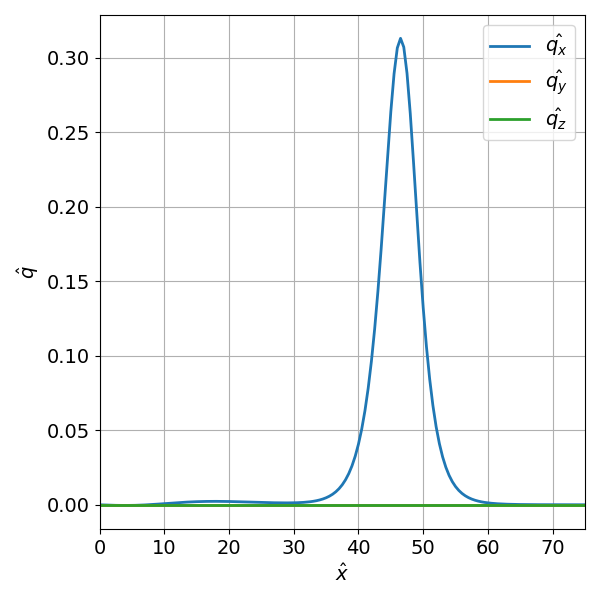
\includegraphics[width=14cm]{plots/problem_c.png}
    \caption{\centering Plot of normalized heat flux $\hat{q}$ in the $x$, $y$, and $z$ directions with respect to distance $\hat{x}$ for times $\hat{t} = 40$ after the main shock has reflected from the wall using inlet speed $\hat{u} = -1$.}
    \label{problem_c}
\end{figure}
The plot of the normalized heat flux in the $x$ direction is a spike between $\hat{x} = 40$ and $\hat{x} = 50$. The value of the normalized heat flux peak is $0.32$. This plot makes sense in the fact that the shock is the main driver for heat raise in the region behind the reflected shock. A shock passes through a region and heats it up, raising the temperature and the number density of the region behind the shock as well. It can also be seen that in the plot, there is a slight heat flux that deviates from 0 in the region behind the shock at $\hat{x} = 20$. This can be attributed to the fact that the domain behind the shock has not settled completely towards equilibrium, causing a slight wobble with the heat flux. From the plots of $\hat{q}_y$ and $\hat{q}_z$, it can be confirmed that the heat fluxes are 0. The flow problem is in one dimension, and it is expected from literature that the heat fluxes are 0 in dimensions other than in $x$.
\clearpage
\subsubsection{Scaled Pressure and Stress Tensor Component Profiles (Part D)}
\begin{figure}[hbt!]
    \centering
    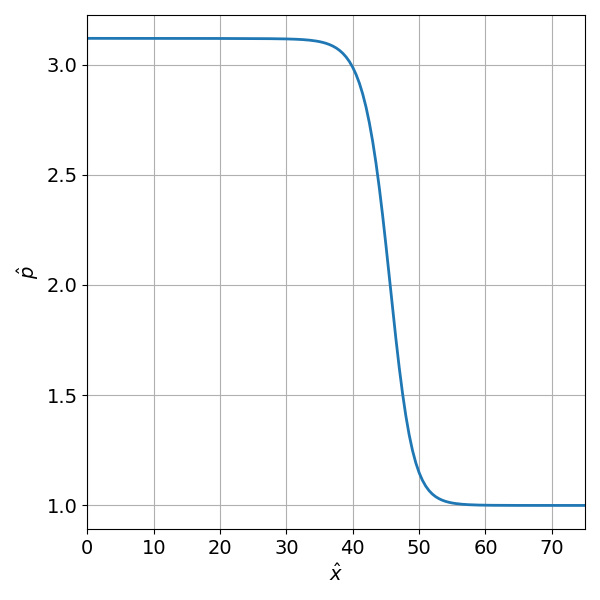
\includegraphics[width=14cm]{plots/problem_d_p.png}
    \caption{\centering Plot of normalized pressure $\hat{p}$ with respect to distance $\hat{x}$ for times $\hat{t} = 40$ after the main shock has reflected from the wall using inlet speed $\hat{u} = -1$.}
    \label{problem_d_p}
\end{figure}
It is shown that the ratio between both the normalized pressures behind and ahead of the shock has settled to a value of 3.25. It is expected that within the shock-tube, the total pressure would decrease but the static pressure would increase due to the normal shock. It is surprising that since the pressure is a function of both number density and temperature $\hat{p} = \hat{n}\hat{T}$, the pressure value behind the shock remains steady with respect to the distance $\hat{x}$ for $\hat{t} = 40$, while for $\hat{n}$ and $\hat{T}$ with respect to the distance $\hat{x}$ is slightly not constant behind the shock. It should be expected that there would be some variation in the value of the normalized pressure $\hat{p}$ behind the shock moving further away from the wall.

\clearpage
\begin{figure}[hbt!]
    \centering
    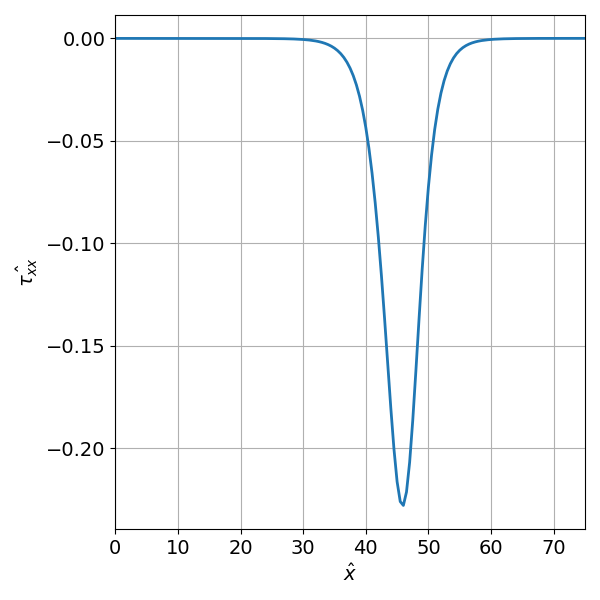
\includegraphics[width=14cm]{plots/problem_d_tau_xx.png}
    \caption{\centering Plot of normalized viscous stresses $\hat{\tau}_{11}$ with respect to distance $\hat{x}$ for times $\hat{t} = 40$ after the main shock has reflected from the wall using inlet speed $\hat{u} = -1$.}
    \label{problem_d_tau_xx}
\end{figure}
The plot of the normalized viscous stresses in the $11$ direction is a negative spike between $\hat{x} = 40$ and $\hat{x} = 50$. The value of the normalized viscous stress in the $xx$ peak is $-0.23$. This plot makes sense in the fact that the shock is the main driver for the viscous stresses in the flow field. The regions behind and ahead of the flow field have a viscous stress of $0$, meaning that the driver for viscous stress in the flow is caused by the shock itself. 

\clearpage
\subsection{BGK Hard-Sphere Molecules Approximation}
\subsubsection{Density and Temp. Comparisons (Part E)}
\begin{figure}[hbt!]
    \centering
    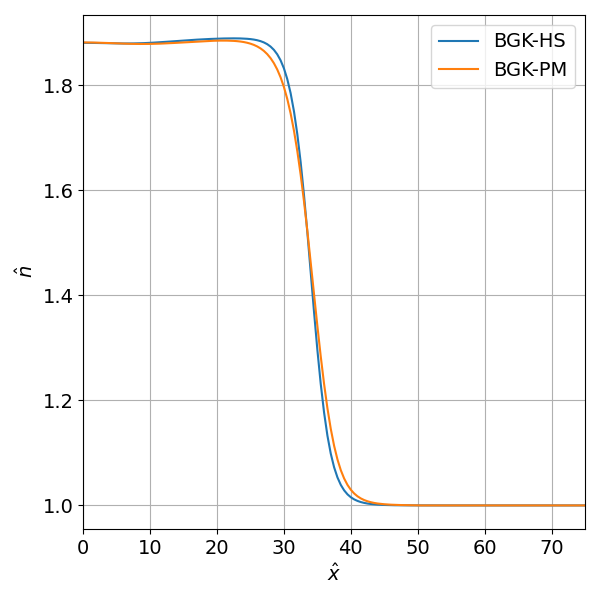
\includegraphics[width=14cm]{plots/problem_e_n.png}
    \caption{\centering Plot of the normalized number density $\hat{n}$ vs. distance from the wall $\hat{x}$ for both BGK pseudo-Maxwell and BGK HS approximations at $\hat{t} = 30$ using inlet speed $\hat{u} = -1$.}
    \label{problem_e_n}
\end{figure}
It can be seen that the hard shell approximation has a steeper slope in $\hat{n}$ vs. $\hat{x}$ to represent the shock than does the pseudo-Maxwell molecules. At $\hat{t} = 30$, we can see that the shock begins for the pseudo-Maxwell approximation nearer to the wall at $\hat{x} = 25$ and ends at around $\hat{x} = 45$, while for the hard shell approximation the shock begins at around $\hat{x} = 28$ and ends around $\hat{x} = 42$. The shock size is much smaller for the hard shell approximation than for the pseudo-Maxwell molecules. It can also be seen that the region behind the shock closest to the wall are identical in value of the number density. However, deviations in the value of the number density are seen moving closer to the shock in the region behind the shockwave. 
\clearpage
\begin{figure}[hbt!]
    \centering
    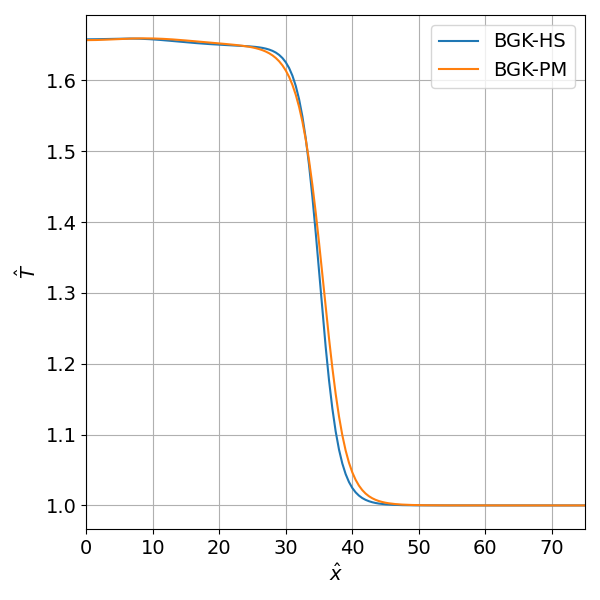
\includegraphics[width=14cm]{plots/problem_e_T.png}
    \caption{\centering Plot of the normalized temperature $\hat{T}$ vs. distance from the wall $\hat{x}$ for both BGK pseudo-Maxwell and BGK HS approximations at $\hat{t} = 30$ using inlet speed $\hat{u} = -1$.}
    \label{problem_e_T}
\end{figure}
Similarly, it can be seen that the hard shell approximation has a steeper slope in $\hat{T}$ vs. $\hat{x}$ to represent the shock than does the pseudo-Maxwell molecules. At $\hat{t} = 30$, we can again see that the shock begins for the pseudo-Maxwell approximation nearer to the wall at $\hat{x} = 25$ and ends at around $\hat{x} = 45$, while for the hard shell approximation the shock begins at around $\hat{x} = 28$ and ends around $\hat{x}= 42$, just like the case of the number density. It can also be seen that the region behind the shock closest to the wall are identical in value of the number density.
\clearpage
\subsubsection{Density and Temp. Comparisons with Different Inlet Speed: $\hat{u} = -2$ (Part F)}
\begin{figure}[hbt!]
    \centering
    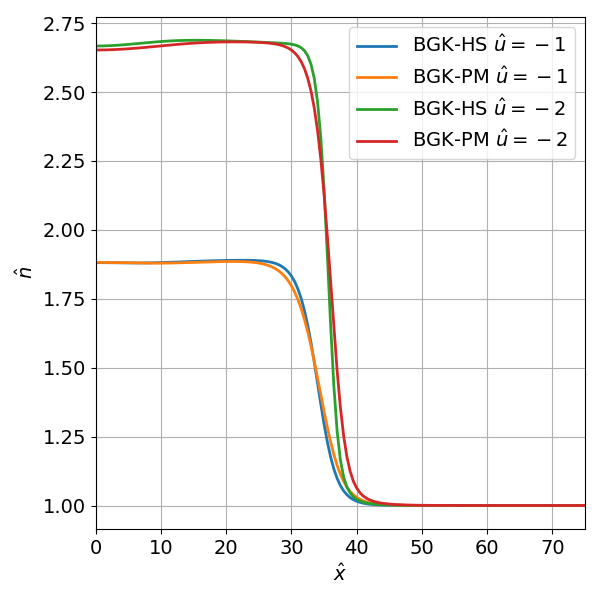
\includegraphics[width=14cm]{plots/problem_f_n.png}
    \caption{\centering Plot of the normalized number density $\hat{n}$ vs. distance from the wall $\hat{x}$ for both BGK pseudo-Maxwell and BGK HS approximations at $\hat{t} = 30$ using inlet speed $\hat{u} = -2$.}
    \label{problem_f_n}
\end{figure}
It can be more evidently seen that the hard shell approximation has a steeper slope in $\hat{n}$ vs. $\hat{x}$ to represent the shock than does the pseudo-Maxwell molecules at a much higher inlet speed. At $\hat{t} = 30$, we can see that the shock begins for the pseudo-Maxwell approximation nearer to the wall at $\hat{x} = 40$ and ends at around $\hat{x} = 55$, while for the hard shell approximation the shock begins at around $\hat{x} = 45$ and ends around $\hat{x} = 50$. Like when the inlet speed is $\hat{u} = -1$, the shock size for  $\hat{u} = -2$ is much smaller for the hard shell approximation than for the pseudo-Maxwell molecules. It can also be seen that the region behind the shock closest to the wall are not identical in value of the number density, unlike the previous case. The hard shell approximation has a higher number density value near the wall in the region behind the shock than do the pseudo-Maxwell molecules. However, when deviating further away from the wall to the area just before the shock, the number densities of the hard shell approximation and the pseudo-Maxwell approximation are the same from $\hat{x} = 30$ to $40$.  
\clearpage
\begin{figure}[hbt!]
    \centering
    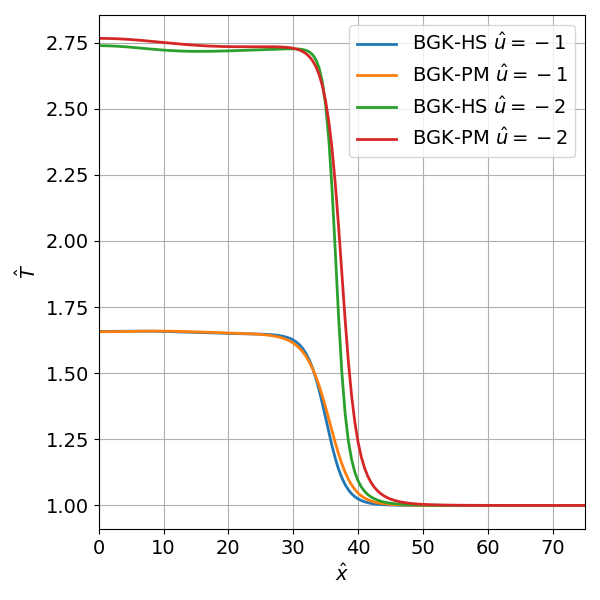
\includegraphics[width=14cm]{plots/problem_f_T.png}
    \caption{\centering Plot of the normalized temperature $\hat{T}$ vs. distance from the wall $\hat{x}$ for both BGK pseudo-Maxwell and BGK HS approximations at $\hat{t} = 30$ using inlet speed $\hat{u} = -2$.}
    \label{problem_f_T}
\end{figure}
In similar fashion, the hard shell approximation has a steeper slope in $\hat{T}$ vs. $\hat{x}$ to represent the shock than does the pseudo-Maxwell molecules at a much higher inlet speed. At $\hat{t} = 30$, we can see that the shock begins for the pseudo-Maxwell approximation at $\hat{x} = 42$ and ends at around $\hat{x} = 55$, while for the hard shell approximation the shock begins at around $\hat{x} = 42$ and ends around $\hat{x} = 51$. Unlike in figure \ref{problem_f_n}, figure \ref{problem_f_T} makes it harder to distinguish between the shock sizes. However, the shock size for  $\hat{u} = -2$ is still much smaller for the hard shell approximation than for the pseudo-Maxwell molecules. It can also be seen that the region behind the shock closest to the wall are not identical in value of the temperature, and more evidently so. The hard shell approximation has a lower number density value near the wall in the region behind the shock than do the pseudo-Maxwell molecules and stays consistently so just before the shock.   
\clearpage
\subsection{ES-BGK Pseudo-Maxwell Molecules Approximation (Part G)}
\begin{figure}[hbt!]
    \centering
    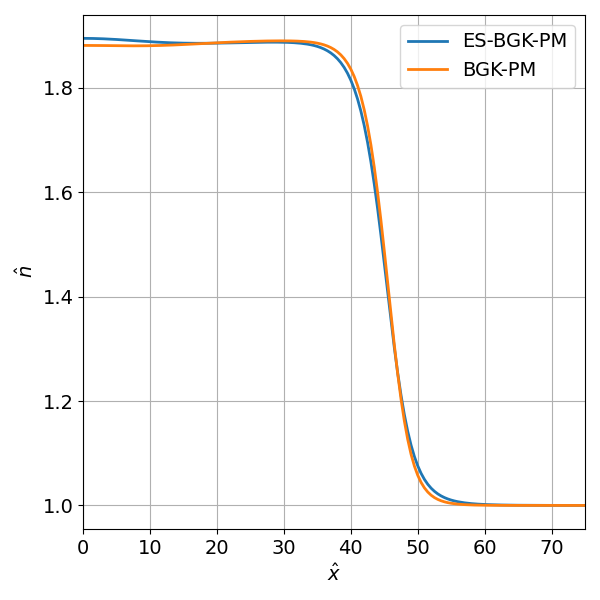
\includegraphics[width=14cm]{plots/problem_g_n.png}
    \caption{\centering Plot of the normalized number density $\hat{n}$ vs. distance from the wall $\hat{x}$ for both BGK pseudo-Maxwell and ES- BGK pseudo-Maxwell approximations at $\hat{t} = 40$ using inlet speed $\hat{u} = -1$.}
    \label{problem_g_n}
\end{figure}
It can be seen that the BGK approximation has a steeper slope in $\hat{n}$ vs. $\hat{x}$ to represent the shock than does the ES-BGK approximation for molecule collisions. At $\hat{t} = 40$, we can see that the shock begins earlier for the ES-BGK molecules and ends later than does the BGK approximation for pseudo-Maxwell molecules. The shock size is much smaller for the BGK approximation than for the ES-BGK approximation. It can also be seen that the region behind the shock closest to the wall are not identical in value of the number density. Rather, nearer to the wall the number densities of the ES-BGK approximation are larger than the BGK approximation, but further away from the wall closer to the shock, the number densities are much larger for the BGK approximation. 
\clearpage
\begin{figure}[hbt!]
    \centering
    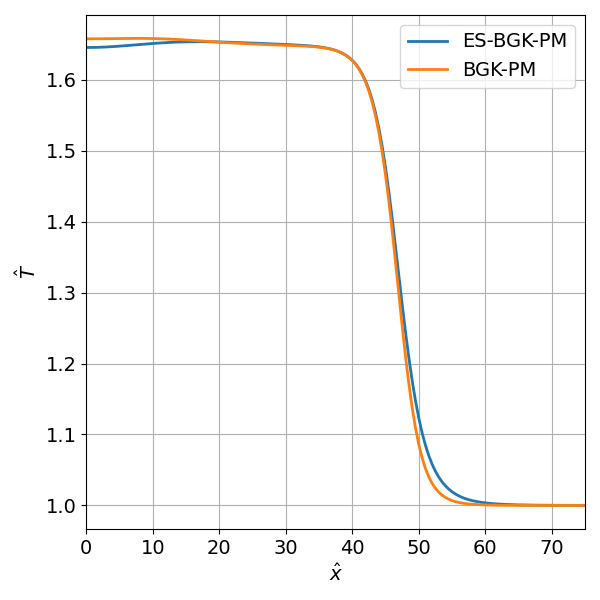
\includegraphics[width=14cm]{plots/problem_g_T.png}
    \caption{\centering Plot of the normalized Temperature $\hat{T}$ vs. distance from the wall $\hat{x}$ for both BGK pseudo-Maxwell and ES- BGK pseudo-Maxwell approximations at $\hat{t} = 40$ using inlet speed $\hat{u} = -1$.}
    \label{problem_g_T}
\end{figure}
It can be seen that the BGK approximation has a steeper slope in $\hat{T}$ vs. $\hat{x}$ to represent the shock than does the ES-BGK approximation for molecule collisions. At $\hat{t} = 40$, we can see that the shock begins at the same time for both BGK and ES-BGK but ends later for the ES-BGK than does the BGK approximation for pseudo-Maxwell molecules. Opposite to the number density plots, nearer to the wall the temperatures of the ES-BGK approximation are smaller than the BGK approximation, but further away from the wall closer to the shock, the number densities are about equal for both approximations. 
\clearpage
\begin{figure}[hbt!]
    \centering
    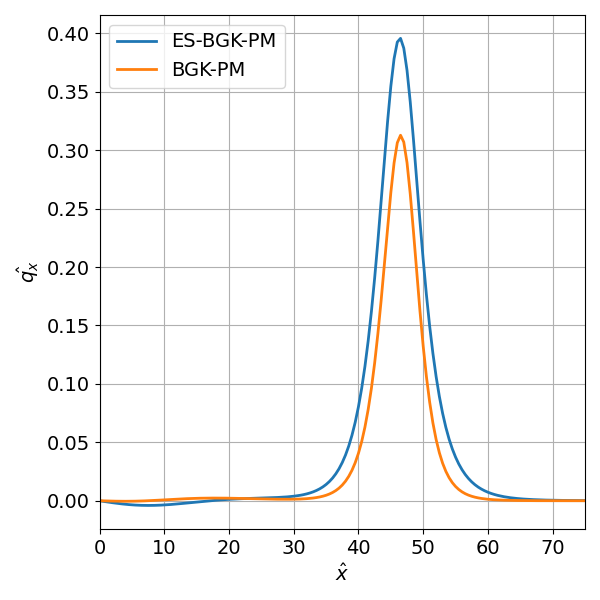
\includegraphics[width=14cm]{plots/problem_g_q_x.png}
    \caption{\centering Plot of the normalized heat flux $\hat{q}_x$ vs. distance from the wall $\hat{x}$ for both BGK pseudo-Maxwell and ES- BGK pseudo-Maxwell approximations at $\hat{t} = 40$ using inlet speed $\hat{u} = -1$.}
    \label{problem_g_q_x}
\end{figure}
From figure \ref{problem_g_n} and figure \ref{problem_g_T}, it can be expected that the ES-BGK approximation would result in a larger shock, and thus result in a larger region for heating, as shown in figure \ref{problem_g_q_x}. The value of $\hat{q}_x$ should be larger with a bigger shock, and thus in figure \ref{problem_g_q_x}, the ES-BGK approximation results in a heat flux peak of around 0.395 and the BGK approximation results in a peak of around 0.31. What is not expected is the negative heat flux at a value $\hat{x} = 10$ for the ES-BGK approximation, which could possibly mean that the solution behind the shockwave has not settled completely at this time step. 
\clearpage
\begin{figure}[hbt!]
    \centering
    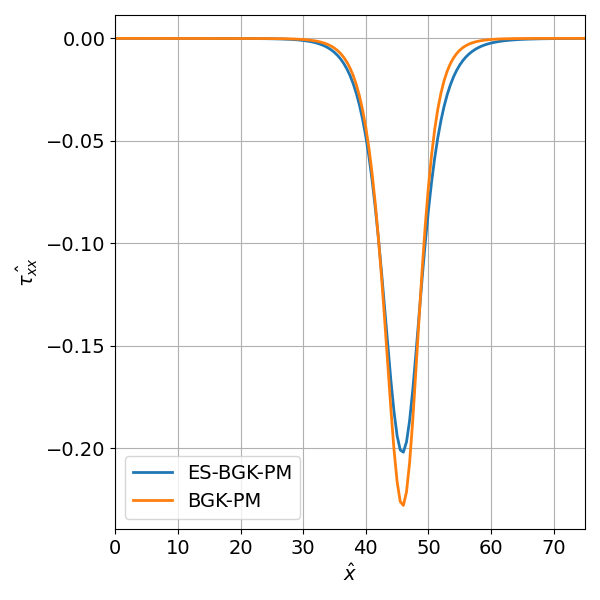
\includegraphics[width=14cm]{plots/problem_g_tau_xx.png}
    \caption{\centering Plot of the normalized viscous stresses $\hat{\tau}_{11}$ vs. distance from the wall $\hat{x}$ for both BGK pseudo-Maxwell and ES- BGK pseudo-Maxwell approximations at $\hat{t} = 40$ using inlet speed $\hat{u} = -1$.}
    \label{problem_g_tau_xx}
\end{figure}
From figure \ref{problem_g_n} and figure \ref{problem_g_T}, it can be expected that the ES-BGK approximation would result in a larger shock, and thus result in a larger region for shear stress, similar to the heat flux, as shown in figure \ref{problem_g_tau_xx}. As the shock is much larger in width, it is expected that the energy would not hold in a wider shock than a narrower shock, so from figure \ref{problem_g_tau_xx} it is shown that the magnitude of the viscous stress is much higher for the BGK approximation than the ES-BGK approximation. Unlike in figure \ref{problem_g_q_x}, the viscous stresses are constant at a value of $0$ behind and ahead of the shock. When viewing the problem on the dimension of the viscous stress, it can be said that the solution behind the shockwave has completely settled. 

\clearpage
\section{Analysis (Part H)}
\subsection{Shockwave Speed \& Uncertainty Analysis}
This analysis will determine the shockwave speed for both BGK and ES-BGK approximations for pseudo-Maxwell molecules from the computations and compare them with the analytical solution for the shockwave speed. The mach number for the analytical solution is determined and using the normal shock relations, the flow properties of pressure, density, and temperature are compared for accuracy. From continuum gas dynamics, the scaled shock velocity $\hat{u}_s$ can be found by determining the positive root in the following equation:
\begin{equation}
    \hat{u}^2_s + \dfrac{3-\gamma}{2} \hat{u}_1 \hat{u}_s - \left[ \gamma +\dfrac{\gamma - 1}{2} \hat{u}^2_1\right] = 0
\end{equation}
Assuming that $\gamma = 5/3$ for a monoatomic gas and $\hat{u}_1 = 1$ for the inflow, the speed of the shock $\hat{u}_s$ can be determined by solving the quadratic equation.
\begin{equation}
    \hat{u}^2_s + \dfrac{3-5/3}{2}(1) \hat{u}_s - \left[5/3 +\dfrac{5/3 - 1}{2} (1)^2\right] = 0
\end{equation}
\begin{equation}
    \hat{u}^2_s +  \dfrac{2}{3}\hat{u}_s - 2 = 0
\end{equation}
Solving the above equation through the quadratic equation, the value of $\hat{u}_s$ becomes:
\begin{equation*}
    \hat{u}_s = 1.11963
\end{equation*}
The solution of the incoming Mach number of the flow is determined by the following equation:
\begin{equation}
    M = \dfrac{\hat{u}_s + \hat{u}_1}{\sqrt{\gamma}} = \dfrac{1.11963 + 1}{\sqrt{5/3}} = 1.6418583
\end{equation}
Using a normal shock calculator, with $\gamma = 5/3$, the ratio of the pressures, densities, and temperatures are the following values:
\begin{equation}
    \dfrac{\hat{p}_2}{\hat{p}_1} =  3.11962334
\end{equation}
\begin{equation}
    \dfrac{\rho_2}{\rho_1} = \dfrac{\hat{n_2}}{\hat{n_1}} = 1.89314697
\end{equation}
\begin{equation}
     \dfrac{\hat{T}_2}{\hat{T}_1} =1.64785058
\end{equation}
\subsection{Analytical vs. Computational Shock Speed}
For measurement of the speed of shock for both BGK and ES-BGK approximations using pseudo-Maxwell molecules, the value of the peak of the heat flux $\hat{q}_x$ will be found at a time $\hat{t}$ and its $\hat{x}$ location measured and located. At the next available time step from the available data, typically at a time-step change of $\Delta\hat{t} = 5$, the value of the peak will be found and its its $\hat{x}$ location also measured. The difference in distance divided by the time-step will be the averaged computational speed of the shock within those time-step ranges.
\begin{equation}
    \hat{u}_{s_{comp}} = \dfrac{\hat{x}_2 - \hat{x}_1}{\Delta\hat{t}}
\end{equation}
The heat flux $\hat{q}_x$ is first plotted for both BGK and ES-BGK models. The locations of these peaks along with the time of occurrence are recorded: 
\begin{figure}[hbt!]
    \centering
    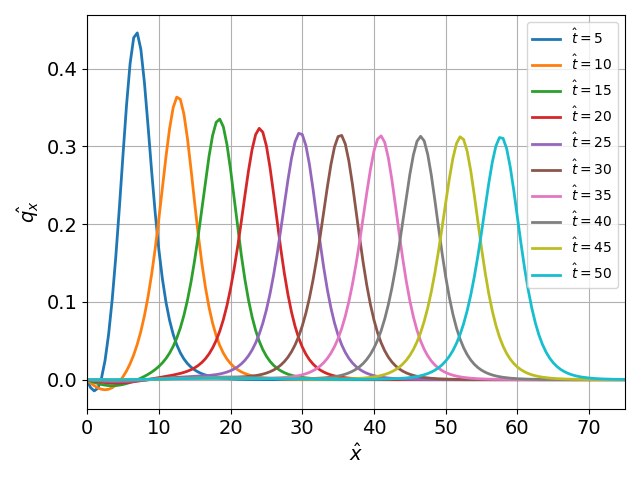
\includegraphics[width=10cm]{plots/problem_speed_BGK.png}
    \caption{\centering Plot of $\hat{q}$ vs. $\hat{t}$ at $0 \leq \hat{t} \leq 50$ using inlet speed $\hat{u} = -1$ with the BGK approximation plotted at every $\Delta\hat{t} = 5$.}
    \label{problem_speed_BGK}
\end{figure}
\begin{figure}[hbt!]
    \centering
    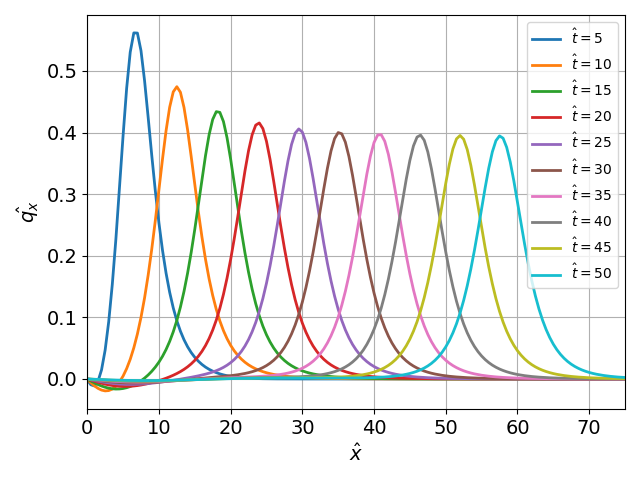
\includegraphics[width=10cm]{plots/problem_speed_ESBGK.png}
    \caption{\centering Plot of $\hat{q}$ vs. $\hat{t}$ at $0 \leq \hat{t} \leq 50$ using inlet speed $\hat{u} = -1$ with the BGK approximation plotted at every $\Delta\hat{t} = 5$.}
    \label{problem_speed_ESBGK}
\end{figure}
\clearpage
Using these plots, the averaged velocity of the shock at every $\Delta\hat{t} = 5$ is shown below in figure \ref{problem_speed_plot} for $0 \leq \hat{t} \leq 50$. 
\begin{figure}[hbt!]
    \centering
    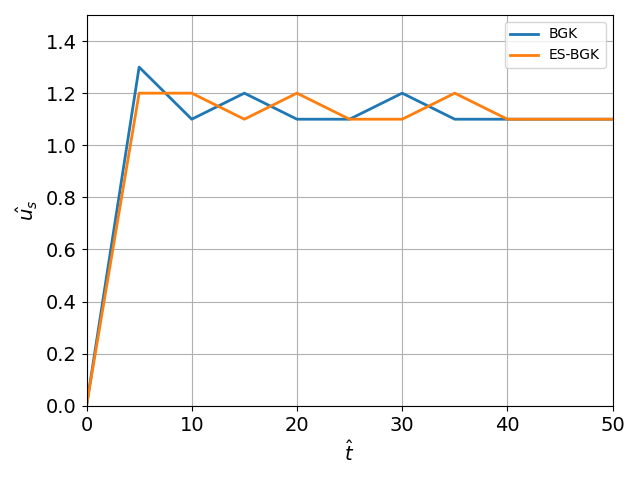
\includegraphics[width=10cm]{plots/problem_speed_BGK_2.png}
    \caption{\centering Plot of $\hat{u}_s$ vs. $\hat{t}$ at $0 \leq \hat{t} \leq 50$ using inlet speed $\hat{u} = -1$ with the BGK and ES-BGK approximations.}
    \label{problem_speed_plot}
\end{figure}

If the average speed is calculated between these time-steps, the average speed for both the BGK approximation and the ES-BGK approximation is $\hat{u}_s = 1.14$. The analytical speed is $\hat{u}_s =1.12$, which represents a $1.785\%$ difference between the computational and analytical solution. At earlier time steps, the BGK solution reaches a peak speed of $\hat{u}_s = 1.3$ before alternating between a speed of $1.2$ and $1.1$. Unlike the BGK solution, the ES-BGK solution does not reach this peak, rather alternating immediately between speeds of $1.1$ and $1.2$ throughout the entire flow period until near the end. After $\hat{t} > 40$, the speeds seem to settle at a value of $1.1$ for both BGK and ES-BGK solutions. 

\clearpage
\subsection{Analytical vs. Computational Flow Ratios}
For each plot of number density, temperature, and pressure for the BGK and ES-BGK pseudo-Maxwell approximations, the values of the flowfield just behind the shock at $\hat{t} = 40$ and from $\hat{x} < 30$ are averaged and recorded as the computational values of the flow field. To obtain the uncertainty in the computational solution, the percentage difference between the analytical solution and the numerical solution is calculated for number density, temperature, and pressure and recorded below.  
\begin{figure}[hbt!]
    \centering
    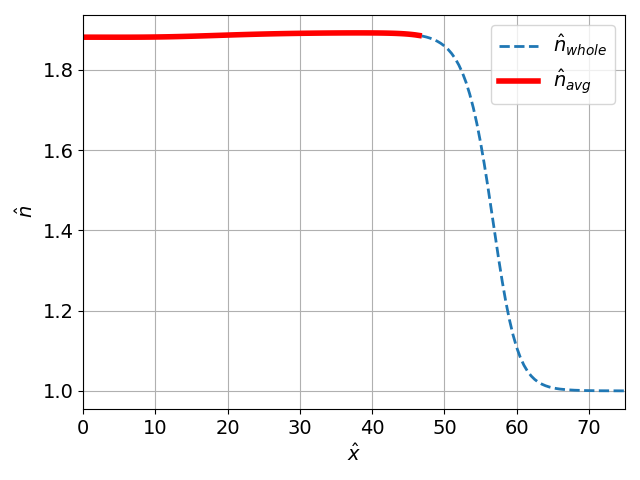
\includegraphics[width=10cm]{plots/problem_h_BGK_n.png}
    \caption{\centering Plot of the selected computational data (in red) for the calculation of the averaged normalized number density using the plot of $\hat{n}$ vs. $\hat{t}$ at $\hat{t} = 50$ using inlet speed $\hat{u} = -1$ with the BGK approximation.}
    \label{problem_h_BGK_n}
\end{figure}
\begin{figure}[hbt!]
    \centering
    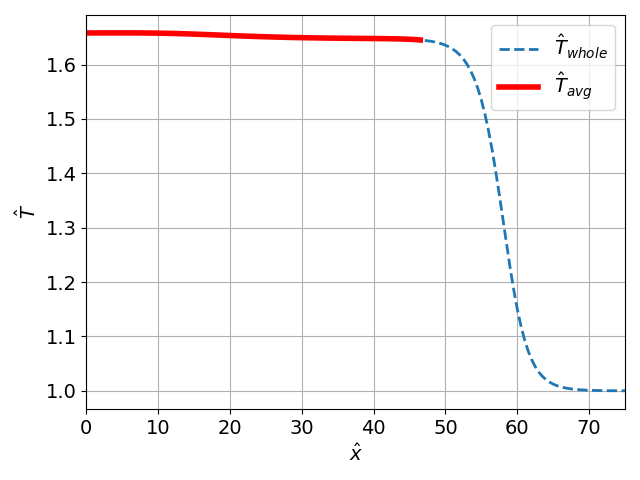
\includegraphics[width=10cm]{plots/problem_h_BGK_T.png}
    \caption{\centering Plot of the selected computational data (in red) for the calculation of the averaged normalized temperature using the plot of $\hat{T}$ vs. $\hat{t}$ at $\hat{t} = 50$ using inlet speed $\hat{u} = -1$ with the BGK approximation.}
    \label{problem_h_BGK_T}
\end{figure}
\begin{figure}[hbt!]
    \centering
    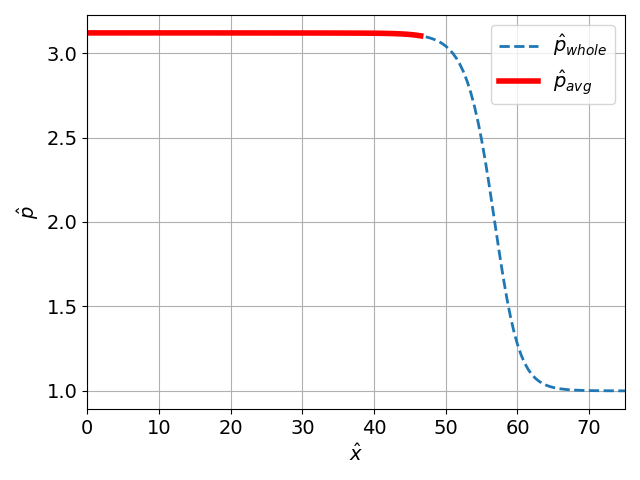
\includegraphics[width=10cm]{plots/problem_h_BGK_p.png}
    \caption{\centering Plot of the selected computational data (in red) for the calculation of the averaged normalized pressure using the plot of $\hat{p}$ vs. $\hat{t}$ at $\hat{t} = 50$ using inlet speed $\hat{u} = -1$ with the BGK approximation.}
    \label{problem_h_BGK_p}
\end{figure}
\begin{figure}[hbt!]
    \centering
    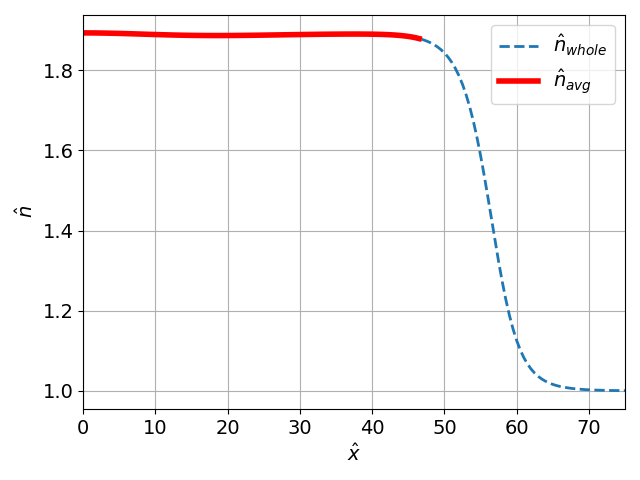
\includegraphics[width=10cm]{plots/problem_h_ESBGK_n.png}
    \caption{\centering Plot of the selected computational data (in red) for the calculation of the averaged normalized number density using the plot of $\hat{n}$ vs. $\hat{t}$ at $\hat{t} = 50$ using inlet speed $\hat{u} = -1$ with the ES-BGK approximation.}
    \label{problem_h_ESBGK_n}
\end{figure}
\begin{figure}[hbt!]
    \centering
    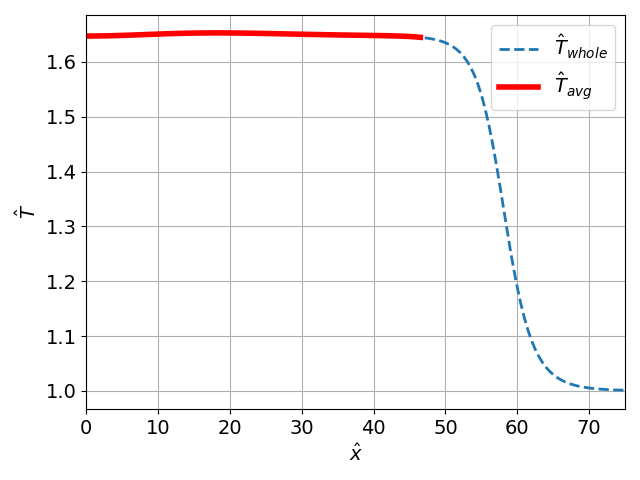
\includegraphics[width=10cm]{plots/problem_h_ESBGK_T.png}
    \caption{\centering Plot of the selected computational data (in red) for the calculation of the averaged normalized temperature using the plot of $\hat{T}$ vs. $\hat{t}$ at $\hat{t} = 50$ using inlet speed $\hat{u} = -1$ with the ES-BGK approximation.}
    \label{problem_h_ESBGK_T}
\end{figure}
\begin{figure}[hbt!]
    \centering
    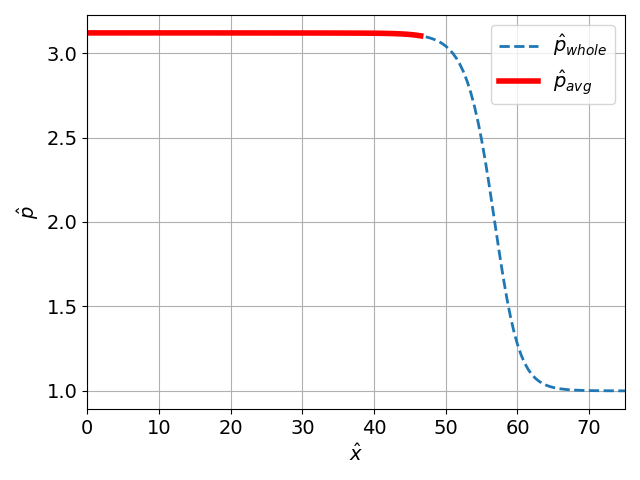
\includegraphics[width=10cm]{plots/problem_h_BGK_p.png}
    \caption{\centering Plot of the selected computational data (in red) for the calculation of the averaged normalized pressure using the plot of $\hat{p}$ vs. $\hat{t}$ at $\hat{t} = 50$ using inlet speed $\hat{u} = -1$ with the ES-BGK approximation.}
    \label{problem_h_ESBGK_p}
\end{figure}
\clearpage
Taking the selected data from each of the flow properties and dividing the averaged data by one returns the desired computational flow properties ratios which is then compared to the analytical solution. The table below represents a summary of the analytical flow ratios, computational flow ratios from the BGK and ES-BGK pseudo-Maxwell approximations, and the percent difference from the analytical solution. 
\begin{table}[h]
\centering
\begin{tabular}{ |c|c|c|c|c|c| } 
\hline
 Ratio & Analytical Solution & BGK & ES-BGK & $\%$ Diff. BGK & $\%$ Diff. ES-BGK \\
\hline
$\hat{n}_2/\hat{n}_1$ & 1.8931 & 1.8869 & 1.8890 & 0.3275$\%$ & 0.2166$\%$ \\
$\hat{T}_2/\hat{T}_1$ & 1.6479 & 1.6524 & 1.6499 & 0.2731$\%$ & 0.1212$\%$ \\
$\hat{p}_2/\hat{p}_1$ & 3.1196 & 3.1180 & 3.1168 & 0.0513$\%$ & 0.0898$\%$ \\
\hline
\end{tabular}
\caption{\centering Flow ratios of normalized number density, pressure, and temperature of the reflected shock from analytical and numerical cases with percent error.}
\label{flow table error}
\end{table}
It can be said from the table shown here that the maximum uncertainty between the BGK solution and the ES-BGK solution for the 1-D reflected shock case is the maximum error found between the three different flow ratios of normalized number density, temperature, or pressure. The BGK solution has an uncertainty of $0.3275\%$ while the ES-BGK solution has an uncertainty of $0.2166\%$. 

\section{Conclusion}

In terms of the 1-D flow for a reflected shock, the work presented in the previous sections reflects on the progress of learning about the Boltzmann equation and how to discretize it to solve a computational program, and coding corresponding models to accurately portray the effects of molecule collisions in non-equilibrium flow. 

In the case of this project, it has been found that the BGK equation is an appropriate model to analyze a flow-field due to a reflected shock. However, although more computationally involved, the ES-BGK model is a slightly better solution technique in comparison to the analytical solutions of the flow ratios across a shock for number density, temperature, and pressure. It has been found that there has also been a noticeable difference in the size of the shock if molecules are modeled as hard spheres versus those that are modeled under pseudo-Maxwell conditions. 

It is suggested that to further test the understanding of the Boltzmann equation and the BGK and ES-BGK models, possibly expanding the dimensions of the flow in two dimensions instead of one will help to discover and understand how a reflected normal shock behaves in both $x$ and $y$ dimensions. It will also be beneficial to attempt the same analysis outlined in section 5 for faster inlet conditions in order to know the limits of inlet speeds that the 1 dimensional program can handle. Higher order methods can also be a potential study for further accuracy of the 1-D reflected shock problem, as some aspects, such as the shock speed or negative heat flux, raise some concerns about the validity of the numerical scheme used for this project. 

\section{Source Files}
The source code, post-processing codes, plots, and deliverables can be found in the following repository: \url{\GitHubLoc}.

\noindent
\clearpage
\bibliographystyle{unsrt}
\bibliography{refs}
\end{document}